\section{Filesystem Management} \label{sec:filesystem_management}
\subsection{Background}
Often in a lab environment, particularly an educational one, users will benefit from having persistent storage so that they may work day to day.   File storage has become less important in recent years because storage is now commercially cheap.  Nowadays, flashdrives that can hold gigabytes of data can be bought for less than one dollar per GB.  In addition, with the advent of cloud storage services, many companies offer free storage online.  Additionally, code repositories not only facilitate filesystem management, but can help with revision archiving.  However, it is still very convenient to have a small amount of storage between computers in a set of labs.  

For network storage, central file servers are the most common.  Some implementations use distributed storage across an entire lab's hard drives.  This method requires a number of security and redundancy considerations and should only be considered if the support staff is able to maintain it.  The central file servers in our environment run Suse Linux and export user home directories with NFS.  

\subsection{NFS Exports}
In the CECS labs, there are 3 file servers each holding 7 hard drives apiece.  Each drive contains home directories for students and faculty members to use daily.  The drives do not have any special configuration and are simply formatted with a standard Linux filesystem.  Each drive is exported via NFS and its exports are only available within CECS lab subnets.  Because of this, we can set the exports to run in insecure mode for compatibility reasons.  We also export with "root\_squash" enabled for all but one subnet.  This prevents an attacker who may have gained root privileges from damaging or stealing all of the files held.  All of this is configured in the "/etc/exports" configuration file on each fileserver.  The simplicity of the configuration has made this system run well for roughly a decade.  Most issues arise from hard drive failures and client configurations.

\subsection{Home Directory Changes}
Although "root\_squash" is useful for preventing possible disasters, "no\_root\_squash" is highly useful for fixing things affecting all students.  For example, when updating between the Linux distributions Fedora to Ubuntu, students still kept the same home directory with the same set of configuration files.  Files that functioned in Fedora broke various features of Ubuntu (most often with window managers).  These file issues are consistently the same with most students. Students can be given instructions, perhaps on the support FAQ, on how to fix issues on their own, but that inevitably leads to many emails to tech support.  Instead, it is useful to have a server or small subnet that has permission to mount student home directories on file servers with "no\_root\_squash."  That way, root can then make edits on all student homes at once via a script.  This script needs to have a lot of checks in place to ensure that it fixes the problem without interfering with other processes.  It also needs highly verbose logging to figure out if anything went wrong.  In its simplest form, this script would just loop through a list of affected student home directories, change directory (cd) to each of them, and run the necessary commands to fix the issue.  A copy of a simple script can be found in Appendix~\ref{ap:lab_maintenance}.

\subsection{Disk Quotas}
Total space for network storage is highly limited in the CECS labs.  Although hard drives have come down in price considerably, with almost 1500 accounts at any given time, a disk quota is necessary.  We set a conservative disk quota of 512 megabytes (MB) for each student and 1 GB for each faculty member.  This may seem small considering the price per GB, but students write code in text files.  They are not doing heavy picture or video editing, so that amount of space has been sufficient so far.  However, we recently noticed that web pages are are becoming larger and browsers are caching more as a result.  Mozilla Firefox in particular now sets its cache limit at 1 GB.  Thus, students are filling up their quotas quickly just by visiting websites.  We have modified the cache in browsers to an older 50 MB limit, but we realize our file servers will need to be upgraded in the next couple of years to keep up with increasingly larger files.  Typically, when the fileservers collectively become more than half full, we begin to worry about space.  

\subsection{Automount}
We use the automount tool on our workstations and servers to mount file shares from our core fileservers.  The automounter has several advantages over the classic method of relying on the file system table (fstab).  The fstab mounts immediately from when the /etc/fstab is read on system startup.  This uses system resources when a mount is not being utilized.  In addition, if a mount fails, it will not remount until either a system administrator (sysadmin) remounts it manually or the system restarts.  The automounter addresses both these issues.  It runs as a daemon in the background and waits for NFS requests by other processes.  It handles the given request and only mounts the file share that it needs to.  In addition, if the mount fails for some reason, it actively attempts to mount again in case there was a random network issue.  The /etc/auto.master configuration file governs the automounter's behavior.

\subsection{Backups}
We have two stages of backups.  One backup is done nightly to a set of file server clones.  These clones have the same hard drive and export configurations as the main file servers.  Though it has never been necessary, theoretically, if a file server goes down, we need only change the hostname of the backup to get it up and running again.  The other backup is done every Saturday to a set of hard drive arrays attached via a Small Computer System Interface (SCSI) cable.  Figure~\ref{fig:FileserverLayout} shows our fileservers and backup fileservers.

\begin{figure}
  \begin{center}
    \scalebox{0.7}{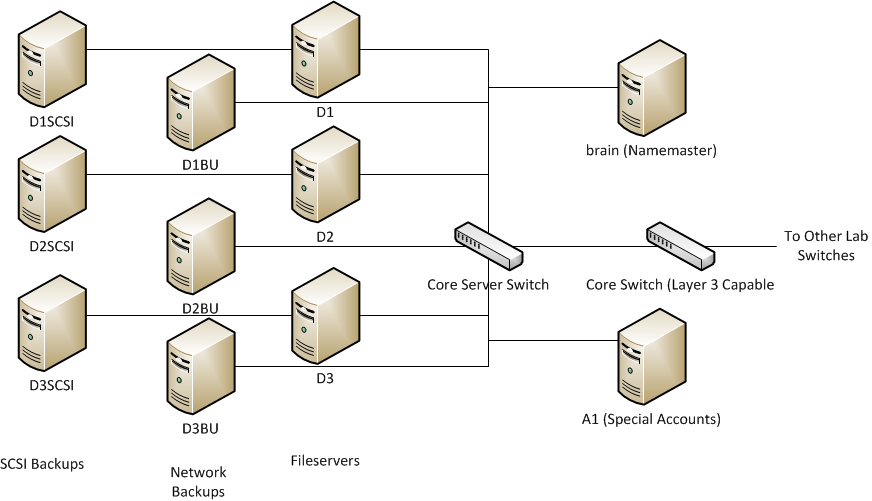
\includegraphics{../figures/FileserverLayout.png}} 
  \end{center}
  \caption{Core fileserver layout.}
  \label{fig:FileserverLayout}
\
\vskip1pt
\
\vskip1pt
\
\end{figure}


Both backups are done with the tar command to keep things simple.  Because this system is so uncomplicated, it is simple to maintain and troubleshoot.  Students are able restore files from backup by running the "retrieve" command and restore their entire home directory with the "shotgun" script.\footnote{A copy of the shotgun script can be found in Appendix~\ref{ap:lab_maintenance}.}

Though they do require periodic checks by our technicians, their simplicity makes our file servers the most stable point of our environment.  Unfortunately, due to higher space demands, their current capacity is quickly becoming insufficient.  Likely, once decommissioned, we will have no more file storage unless funding is appropriated for more space.  Without file storage, students will have to procure their own space either from their own media or from an online provider.  In either case, they will also have to find their own backup procedure.  Whatever solution they find, it will most likely not be seamless with our environment. 

\subsection{Student Media}
Students can also use their own USB drives to store their files if the space provided by us is insufficient.  Student media drives, however, pose a security risk. Upon insertion of a memory drive into a Universal Serial Bus (USB) port, Windows has the tendency to look onto the drives for drivers and may run malicious code that could infect the workstations.  This has become less of an issue now that Microsoft has finally implemented security measures.  On Linux workstations, we simply do not allow any files on the drives to execute.  We also prevent the drives from being mounted with administrative privileges.  Students can use the "pmount" and "pumount" commands to mount/unmount the drives as normal users without privileges.  This also forces them to mount manually and prevents exploits of an automatic USB mounting system.  

\subsection{Malware}
We occasionally receive reports of malware on our lab workstations.  We have powerful anti-virus software but this does not prevent all pieces of code from running.  Many instances are just programs in memory that disappear as soon as a student logs off.  Others may just reside in temporary files that are easily cleared.  Regardless, we run an environment that teaches programming.  We cannot prevent students from running malicious code intentionally or unintentionally.  We do, however, have the ability to track which students are repeat offenders.  We have the authority to temporarily reduce the ability to do further damage by locking accounts.  Further action can be taken only by involving the faculty, the department administrators, or even university administrators in the event of extreme wrongdoing. 
